\let\negmedspace\undefined
\let\negthickspace\undefined
\documentclass[journal,12pt,onecolumn]{IEEEtran}
\usepackage{cite}
\usepackage{amsmath,amssymb,amsfonts,amsthm}
\usepackage{algorithmic}
\usepackage{graphicx}
\graphicspath{{./figs/}}
\usepackage{textcomp}
\usepackage{xcolor}
\usepackage{txfonts}
\usepackage{listings}
\usepackage{enumitem}
\usepackage{mathtools}
\usepackage{gensymb}
\usepackage{comment}
\usepackage{caption}
\usepackage[breaklinks=true]{hyperref}
\usepackage{tkz-euclide} 
\usepackage{listings}
\usepackage{gvv}                                        
%\def\inputGnumericTable{}                                 
\usepackage[latin1]{inputenc}     
\usepackage{xparse}
\usepackage{color}                                            
\usepackage{array}                                            
\usepackage{longtable}                                       
\usepackage{calc}                                             
\usepackage{multirow}
\usepackage{multicol}
\usepackage{hhline}                                           
\usepackage{ifthen}                                           
\usepackage{lscape}
\usepackage{tabularx}
\usepackage{array}
\usepackage{float}
\newtheorem{theorem}{Theorem}[section]
\newtheorem{problem}{Problem}
\newtheorem{proposition}{Proposition}[section]
\newtheorem{lemma}{Lemma}[section]
\newtheorem{corollary}[theorem]{Corollary}
\newtheorem{example}{Example}[section]
\newtheorem{definition}[problem]{Definition}
\newcommand{\BEQA}{\begin{eqnarray}}
\newcommand{\EEQA}{\end{eqnarray}}
\newcommand{\define}{\stackrel{\triangle}{=}}
\theoremstyle{remark}
\newtheorem{rem}{Remark}

\begin{document}
\title{
ASSIGNMENT 2: GATE 2014  \\
PI : PRODUCTION \& INDUSTRIAL ENGINEERING}
\author{EE25BTECH11054 - S. Harsha Vardhan Reddy}
\maketitle
\renewcommand{\thefigure}{\theenumi}
\renewcommand{\thetable}{\theenumi}
\begin{enumerate}
    \item Choose the most appropriate word from the options given below to complete the following sentence.
    
    A person suffering from Alzheimer's disease \underline{\hspace{2cm}} short-term memory loss.
    
    \hfill{\brak{\text{GATE PI 2014}}}
    \begin{enumerate}
        \begin{multicols}{2}
            \item experienced
            \item has experienced
            \item is experiencing
            \item experiences
        \end{multicols}
    \end{enumerate}

    \item Choose the most appropriate word from the options given below to complete the following sentence.
    
    \underline{\hspace{2cm}} is the key to their happiness; they are satisfied with what they have.
    
    \hfill{\brak{\text{GATE PI 2014}}}
    \begin{enumerate}
        \begin{multicols}{4}
            \item Contentment
            \item Ambition
            \item Perseverance
            \item Hunger
        \end{multicols}
    \end{enumerate}

    \item Which of the following options is the closest in meaning to the sentence below?
    
    "As a woman, I have no country."
    
    \hfill{\brak{\text{GATE PI 2014}}}
    \begin{enumerate}
        \item Women have no country.
        \item Women are not citizens of any country.
        \item Women's solidarity knows no national boundaries.
        \item Women of all countries have equal legal rights.
    \end{enumerate}

    \item In any given year, the probability of an earthquake of Magnitude $6$ occurring in the Garhwal Himalayas is $0.04$. The average time between successive occurrences of such earthquakes is \underline{\hspace{2cm}} years.
    
    \hfill{\brak{\text{GATE PI 2014}}}

    \item The population of a new city is $5$ million and is growing at $20\%$ annually. How many years would it take to double at this growth rate?
    
    \hfill{\brak{\text{GATE PI 2014}}}
    \begin{enumerate}
        \begin{multicols}{4}
            \item 3-4 years
            \item 4-5 years
            \item 5-6 years
            \item 6-7 years
        \end{multicols}
    \end{enumerate}

    \item In a group of four children, Som is younger to Riaz. Shiv is elder to Ansu. Ansu is youngest in the group. Which of the following statements is/are required to find the eldest child in the group?
    
    $1$. Shiv is younger to Riaz.
    
    $2$. Shiv is elder to Som.
    
    \hfill{\brak{\text{GATE PI 2014}}}
    \begin{enumerate}
        \item Statement 1 by itself determines the eldest child.
        \item Statement 2 by itself determines the eldest child.
        \item Statements 1 and 2 are both required to determine the eldest child.
        \item Statements 1 and 2 are not sufficient to determine the eldest child.
    \end{enumerate}

    \item Moving into a world of big data will require us to change our thinking about the merits of exactitude. To apply the conventional mindset of measurement to the digital, connected world of the twenty-first century is to miss a crucial point. As mentioned earlier, the obsession with exactness is an artefact of the information-deprived analog era. When data was sparse, every data point was critical, and thus great care was taken to avoid letting any point bias the analysis.
    
    From "BIG DATA" Viktor Mayer-Schonberger and Kenneth Cukier
    
    The main point of the paragraph is:
    
    \hfill{\brak{\text{GATE PI 2014}}}
    \begin{enumerate}
        \item The twenty-first century is a digital world
        \item Big data is obsessed with exactness
        \item Exactitude is not critical in dealing with big data
        \item Sparse data leads to a bias in the analysis
    \end{enumerate}

    \item The total exports and revenues from the exports of a country are given in the two pie charts below. The pie chart for exports shows the quantity of each item as a percentage of the total quantity of exports. The pie chart for the revenues shows the percentage of the total revenue generated through export of each item. The total quantity of exports of all the items is $5$ lakh tonnes and the total revenues are $250$ crore rupees. What is the ratio of the revenue generated through export of Item 1 per kilogram to the revenue generated through export of Item 4 per kilogram?
    
    \begin{figure}[H]
        \centering
        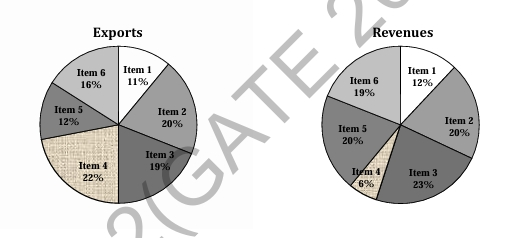
\includegraphics[width=0.8\columnwidth]{q8.png}
        \caption*{}
        \label{fig:q8}
    \end{figure}
    
    \hfill{\brak{\text{GATE PI 2014}}}
    \begin{enumerate}
        \begin{multicols}{4}
            \item $1\colon2$
            \item $2\colon1$
            \item $1\colon4$
            \item $4\colon1$
        \end{multicols}
    \end{enumerate}

    \item X is $1$ km northeast of Y. Y is $1$ km southeast of Z. W is $1$ km west of Z. P is $1$ km south of W. Q is $1$ km east of P. What is the distance between X and Q in km?
    
    \hfill{\brak{\text{GATE PI 2014}}}
    \begin{enumerate}
        \begin{multicols}{4}
            \item $1$
            \item $\sqrt{2}$
            \item $\sqrt{3}$
            \item $2$
        \end{multicols}
    \end{enumerate}

    \item $10\%$ of the population in a town is HIV$^+$. A new diagnostic kit for HIV detection is available; this kit correctly identifies HIV$^+$ individuals $95\%$ of the time, and HIV$^-$ individuals $89\%$ of the time. A particular patient is tested using this kit and is found to be positive. The probability that the individual is actually positive is \underline{\hspace{2cm}}.
    
    \hfill{\brak{\text{GATE PI 2014}}}
\end{enumerate}
\begin{enumerate}

    \item The system of equations, given below, has
    \begin{align*}
        x+2y+4z &= 2 \\
        4x+3y+z &= 5 \\
        3x+2y+3z &= 1
    \end{align*}
    
    \hfill{\brak{\text{GATE PI 2014}}}
    \begin{enumerate}
        \begin{multicols}{2}
            \item a unique solution
            \item two solutions
            \item no solution
            \item more than two solutions
        \end{multicols}
    \end{enumerate}

    \item Directional derivative of $\phi=2xz-y^{2}$, at the point $\brak{1, 3, 2}$, becomes maximum in the direction of
    
    \hfill{\brak{\text{GATE PI 2014}}}
    \begin{enumerate}
        \begin{multicols}{4}
            \item $4i+2j-3k$
            \item $4i-6j+2k$
            \item $2i-6j+2k$
            \item $4i-6j-2k$
        \end{multicols}
    \end{enumerate}

    \item A metallic sphere of $0.1$ m diameter has a thermal conductivity of $10$ W/m-K. If the fluid flowing around it has a heat transfer coefficient of $10~\text{W/m}^2\text{-K}$ and thermal conductivity of $0.4~\text{W/m-K}$, the value of Biot number is \underline{\hspace{2cm}}.
    
    \hfill{\brak{\text{GATE PI 2014}}}

    \item A quantitative measure of maintainability is
    
    \hfill{\brak{\text{GATE PI 2014}}}
    \begin{enumerate}
        \begin{multicols}{2}
            \item Downtime
            \item Mean Time Between Failure
            \item Mean Time To Repair
            \item System availability
        \end{multicols}
    \end{enumerate}

    \item Which one of the following techniques is used to analyze the cause and effect of product failure?
    
    \hfill{\brak{\text{GATE PI 2014}}}
    \begin{enumerate}
        \begin{multicols}{2}
            \item Quality Function Deployment
            \item Fault Tree Analysis
            \item Value Analysis
            \item Failure Mode and Effect Analysis
        \end{multicols}
    \end{enumerate}

    \item As the product passes through different stages of product life cycle, the product variety
    
    \hfill{\brak{\text{GATE PI 2014}}}
    \begin{enumerate}
        \begin{multicols}{2}
            \item increases
            \item decreases and then increases
            \item remains the same
            \item decreases
        \end{multicols}
    \end{enumerate}

    \item A machine has been purchased for Rs. $100,000$ and its useful life is estimated to be $10$ years. Its scrap value at the end of $10$ years is estimated as Rs. $20,000$. If the depreciation is determined using the declining balance method, the value of depreciation \brak{\text{in Rs.}} during the first year is \underline{\hspace{2cm}}.
    
    \hfill{\brak{\text{GATE PI 2014}}}

    \item A company wants to determine the proportion of time workers are idle. In a pilot study, the proportion of idle time was found to be $0.16$. If the company wants to be $95\%$ confident \brak{\text{z-value}=1.96} that the estimated value is within $0.03$ of the true proportion, the number of observations required in the study should be \underline{\hspace{2cm}}.
    
    \hfill{\brak{\text{GATE PI 2014}}}

    \item A manufacturing plant, working in $2$ shifts of $8$ hrs each, produces $30,000$ switch boards using a set of $7$ workstations in series. The cycle time, in seconds, is \underline{\hspace{2cm}}.
    
    \hfill{\brak{\text{GATE PI 2014}}}

    \item A simple random sample of $100$ observations was taken from a large population. The sample mean and the standard deviation were determined to be $80$ and $12$, respectively. The standard error of mean is \underline{\hspace{2cm}}.
    
    \hfill{\brak{\text{GATE PI 2014}}}
    
    \item The diameter of a shaft must be within a tolerance of $0.02$ of the nominal diameter. Which control chart is useful to determine that the process is in statistical control?
    
    \hfill{\brak{\text{GATE PI 2014}}}
    \begin{enumerate}
        \begin{multicols}{4}
            \item p chart
            \item c chart
            \item $\overline{X}$ and R chart
            \item U chart
        \end{multicols}
    \end{enumerate}
    
    \item Which one of the following is not a characteristic of JIT manufacturing system?
    
    \hfill{\brak{\text{GATE PI 2014}}}
    \begin{enumerate}
        \begin{multicols}{2}
            \item Reduction of lot sizes
            \item Efficient use of buffer inventory
            \item Small but frequent deliveries
            \item Higher productivity
        \end{multicols}
    \end{enumerate}
    
    \item Relationship between Young's Modulus \brak{E}, Shear Modulus \brak{G}, and Poisson's Ratio \brak{\mu}, for a material obeying the Hooke's Law, is
    
    \hfill{\brak{\text{GATE PI 2014}}}
    \begin{enumerate}
        \begin{multicols}{4}
            \item $E=\frac{G}{\brak{2+\mu}}$
            \item $E=\frac{2G}{\brak{1+\mu}}$
            \item $E=G\brak{1+\mu}$
            \item $E=2G\brak{1+\mu}$
        \end{multicols}
    \end{enumerate}

    \item For a metal alloy, which one of the following descriptions relates to the stress-relief annealing process?
    
    \hfill{\brak{\text{GATE PI 2014}}}
    \begin{enumerate}
        \item Heating the workpiece material above its recrystallization temperature, soaking and then cooling in still air
        \item Heating the workpiece material below its recrystallization temperature, holding for some time and then furnace cooling
        \item Heating the workpiece material up to its recrystallization temperature and then rapid cooling
        \item Heating the workpiece up to its recrystallization temperature and cooling to room temperature alternately for a few cycles
    \end{enumerate}

    \item Generative Approach of Computer Aided Process Planning is NOT based on
    \begin{itemize}
        \item[\brak{i}] part coding using Group Technology
        \item[\brak{ii}] part feature representation
        \item[\brak{iii}] database of standard process plans for part families
        \item[\brak{iv}] geometric modelling
    \end{itemize}
    
    \hfill{\brak{\text{GATE PI 2014}}}
    \begin{enumerate}
        \begin{multicols}{4}
            \item \brak{i} and \brak{ii}
            \item \brak{i} and \brak{iii}
            \item \brak{iii} and \brak{iv}
            \item \brak{i}, \brak{ii} and \brak{iv}
        \end{multicols}
    \end{enumerate}

    \item Which one of the following methods is NOT used for producing metal powders?
    
    \hfill{\brak{\text{GATE PI 2014}}}
    \begin{enumerate}
        \begin{multicols}{2}
            \item Atomization
            \item Sintering
            \item Machining and grinding
            \item Electrolysis
        \end{multicols}
    \end{enumerate}

    \item In an open loop, point-to-point controlled CNC drilling machine, a stepper motor, producing $200$ angular steps per revolution, drives the table of a drilling machine by one angular step per each pulse generated by a pulse generator \brak{\text{shown in figure}}. Each angular step moves the table by one Basic Length Unit \brak{BLU} along X axis with a lead screw having a pitch of $4$ mm. If the frequency of pulse generator is doubled, the BLU will
    \begin{figure}[H]
        \centering
        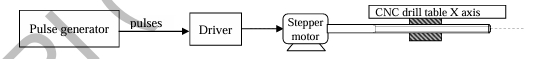
\includegraphics[width=0.7\columnwidth]{q17.png}
        \caption*{}
        \label{fig:q17}
    \end{figure}
    
    \hfill{\brak{\text{GATE PI 2014}}}
    \begin{enumerate}
        \begin{multicols}{2}
            \item become double of previous value
            \item become half of previous value
            \item remain the same
            \item become zero
        \end{multicols}
    \end{enumerate}

    \item A spindle speed of $300$ rpm and a feed of $0.3$ mm/revolution are chosen for longitudinal turning operation on an engine lathe. In finishing pass, roughness on the work surface can be reduced by
    
    \hfill{\brak{\text{GATE PI 2014}}}
    \begin{enumerate}
        \begin{multicols}{2}
            \item reducing the spindle speed
            \item increasing the spindle speed
            \item reducing the feed of tool
            \item increasing the feed of tool
        \end{multicols}
    \end{enumerate}

    \item Chills are used in casting moulds to
    
    \hfill{\brak{\text{GATE PI 2014}}}
    \begin{enumerate}
        \begin{multicols}{2}
            \item achieve directional solidification
            \item reduce the roughness of top surface of the cast product
            \item increase the solidification time
            \item reserve excess molten metal
        \end{multicols}
    \end{enumerate}

    \item A moving mandrel is used in
    
    \hfill{\brak{\text{GATE PI 2014}}}
    \begin{enumerate}
        \begin{multicols}{4}
            \item wire drawing
            \item forging
            \item tube drawing
            \item bending
        \end{multicols}
    \end{enumerate}
    
    \item Brazing and Soldering are
    
    \hfill{\brak{\text{GATE PI 2014}}}
    \begin{enumerate}
        \item plastic joining methods
        \item liquid state joining methods
        \item solid state joining methods
        \item solid/liquid state joining methods
    \end{enumerate}
    
    \item Match the following
    \begin{table}[H]
        \centering
        \caption*{}
        \label{tab:q22}
        \begin{tabular}{ll|ll}
            \hline
            \multicolumn{2}{c|}{\textbf{Group I \brak{\text{Mechanism}}}} & \multicolumn{2}{c}{\textbf{Group II \brak{\text{Machines}}}} \\
            \hline
            P & Quick return & 1 & Lathe \\
            Q & Apron & 2 & Shaping \\
            R & Intermittent indexing & 3 & Gear hobbing \\
            S & Differential mechanism & 4 & Milling \\
            \hline
        \end{tabular}
    \end{table}
    
    \hfill{\brak{\text{GATE PI 2014}}}
    \begin{enumerate}
        \begin{multicols}{2}
            \item P1-Q2-R4-S3
            \item P2-Q1-R4-S3
            \item P4-Q1-R2-S3
            \item P2-Q3-R1-S4
        \end{multicols}
    \end{enumerate}

    \item Reaming is a process used for
    
    \hfill{\brak{\text{GATE PI 2014}}}
    \begin{enumerate}
        \item creating a circular hole in metals
        \item cutting a slot on the existing hole surface
        \item finishing an existing hole surface
        \item making non-circular holes in metals
    \end{enumerate}

    \item Find the correct combination of manufacturing processes to produce the part, shown in figure, from a blank \brak{\text{holes shown are with square and circular cross-sections}}.
    
    \begin{figure}[H]
        \centering
        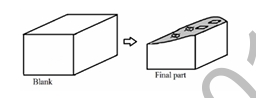
\includegraphics[width=0.7\columnwidth]{q24.png}
        \caption*{}
        \label{fig:q24}
    \end{figure}
    
    \hfill{\brak{\text{GATE PI 2014}}}
    \begin{enumerate}
        \item Drilling and milling on column and knee type universal milling machine
        \item Die-sinking and CNC Wire-cut EDM process
        \item Die-sinking and CNC drilling
        \item CNC Wire-cut EDM process only
    \end{enumerate}

    \item In an open die forging, a circular disc is gradually compressed between two flat platens. The exponential decay of normal stress on the flat face of the disc, from the center of the disc towards its periphery, indicates that
    
    \hfill{\brak{\text{GATE PI 2014}}}
    \begin{enumerate}
        \item there is no sticking friction anywhere on the flat face of the disc
        \item sticking friction and sliding friction co-exist on the flat face of the disc
        \item the flat face of the disc is frictionless
        \item there is only sticking friction on the flat face of the disc
    \end{enumerate}

    \item If $\varphi = 2x^3y^2z^4$ then $\nabla^2\varphi$ is 

    \hfill{\brak{\text{GATE PI 2014}}}

    \begin{enumerate}
    \item $12xy^2z^4 + 4x^2z^4 + 20x^3y^3z^3$
    \item $2x^2y^2z + 4x^3z^ + 24x^3y^2z^2$
    \item $12xy^2z^4 + 4x^3z^4 + 24x^3y^2z^2$
    \item $4xy^2z + 4x^2z^4 + 24x^3y^2z^2$
    \end{enumerate}

    \item Using the Simpson's $1/3$rd rule, the value of $\int_1^5 ydx$ computed, for the data given below, is \underline{\hspace{2cm}}.
    
    \begin{table}[H]
        \centering
        \caption*{}
        \label{tab:q27}
        \begin{tabular}{c|ccc}
            \hline
            x & 1 & 3 & 5 \\
            \hline
            y & 2 & 6 & 4 \\
            \hline
        \end{tabular}
    \end{table}
    
    \hfill{\brak{\text{GATE PI 2014}}}
    
    \item If the equation $\sin\brak{x} = x^2$ is solved by Newton Raphson's method with the initial guess of $x=1$, then the value of x after $2$ iterations would be \underline{\hspace{2cm}}.
    
    \hfill{\brak{\text{GATE PI 2014}}}
    
    \item If $2$ kg mass of water, with a specific heat of $4.18$ kJ/kg-K, is heated from $20\degree$C to $40\degree$C in an open container, then the change in entropy of water, in kJ/K, is \underline{\hspace{2cm}}.
    
    \hfill{\brak{\text{GATE PI 2014}}}
    
    \item A gas at a pressure of $500$ kPa and volume of $0.75\text{m}^3$ is contained in a cylinder-piston assembly. When the piston moves slowly in the cylinder, the pressure inside the cylinder varies as $V^{-1.2}$. If the final volume of gas becomes doubled, then the work done by the gas, in kJ, is \underline{\hspace{2cm}}.
    
    \hfill{\brak{\text{GATE PI 2014}}}
    
    \item Two geometrically identical metallic bars are joined end to end \brak{\text{as shown in Fig.}}. Bars P and Q have thermal conductivities of $5$ W/m-K and $10$ W/m-K respectively. The free end of the Bar P is kept at $40\degree$C, while that of Bar Q is at $10\degree$C. The junction temperature \brak{\text{in }\degree\text{C}} for steady state heat flow is \underline{\hspace{2cm}}.
    
    \begin{figure}[H]
        \centering
        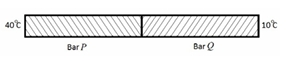
\includegraphics[width=0.8\columnwidth]{q31.png}
        \caption*{}
        \label{fig:q31}
    \end{figure}
    
    \hfill{\brak{\text{GATE PI 2014}}}
    
    \item A metallic sphere of $1$ kg mass, with surface area of $0.0314 \text{ m}^2$, is maintained at an initial temperature of $50\degree$C. The fluid circulating around the sphere is maintained at a temperature of $10\degree$C. Specific heat of metallic sphere is $314$ J/kg-K and the heat transfer coefficient between the fluid and the sphere is $10$ W/m$^2$-K. The time taken \brak{\text{in seconds}} for the sphere to cool down to $20\degree$C is \underline{\hspace{2cm}}.
    
    \hfill{\brak{\text{GATE PI 2014}}}

    \item An element, shown below, is subjected to stresses: $\sigma_x = 5 \text{ kN/mm}^2$, $\sigma_y = 3 \text{ kN/mm}^2$ and $\tau = 1 \text{ kN/mm}^2$. The magnitudes and direction of principal stresses $\sigma_1$, $\sigma_2$ \brak{\text{in kN/mm$^2$}} and $\phi$ \brak{\text{in degrees}} are
    
    \begin{figure}[H]
        \centering
        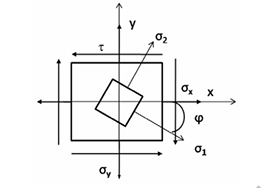
\includegraphics[width=0.5\columnwidth]{q33.png}
        \caption*{}
        \label{fig:q33}
    \end{figure}
    
    \hfill{\brak{\text{GATE PI 2014}}}
    \begin{enumerate}
        \begin{multicols}{2}
            \item $5.41, 2.58, -22.5$
            \item $5.41, 2.58, -45$
            \item $5.0, 3.0, -22.5$
            \item $4.0, 4.0, -22.5$
        \end{multicols}
    \end{enumerate}

    \item Each axis of NC machine is driven by a stepper motor drive with a lead screw. The pitch of lead screw is p mm. The step angle of stepper motor per pulse input is $\alpha$ degrees/pulse. The ratio of gear drive in stepper motor drive is g \brak{\text{number of turns of the motor for each single turn of the lead screw}}. The number of pulses required to achieve a linear movement of x mm is
    
    \hfill{\brak{\text{GATE PI 2014}}}
    \begin{enumerate}
        \begin{multicols}{4}
            \item $\frac{360gx}{p\alpha}$
            \item $\frac{360g}{\alpha xp}$
            \item $\frac{360xp}{g\alpha}$
            \item $\frac{360\alpha g}{xp}$
        \end{multicols}
    \end{enumerate}

    \item A uniformly distributed load \brak{q} of $1500$ N/m is applied on a simply supported beam LMN with an overhang of $0.5$ m. Which one of the following statements is FALSE?
    
    \begin{figure}[H]
        \centering
        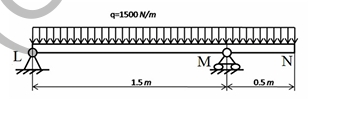
\includegraphics[width=\columnwidth]{q35.png}
        \caption*{}
        \label{fig:q35}
    \end{figure}
    
    \hfill{\brak{\text{GATE PI 2014}}}
    \begin{enumerate}
        \item Reaction forces at L and M are 1 kN and 2 kN
        \item Bending moment is zero at the points L, N and at a point in between L and M
        \item The bending moment is zero at points L and N only
        \item The shear force is zero at points L, N and at a point in between L and M
    \end{enumerate}

    \item A CNC instruction G91G01X30Y40F100 commands the movement of tool along the path at a feed rate of $100$ mm/min \brak{\text{G91- incremental format and G01- linear interpolation}}. The feed rate of the tool \brak{\text{in mm/min}} along the X axis will be \underline{\hspace{2cm}}.
    
    \hfill{\brak{\text{GATE PI 2014}}}

    \item Elastic moduli of a fibre reinforced plastic composite and fibres are $200$ GPa and $400$ GPa, respectively. The longitudinal fibres are taking up $50\%$ of the load. Assuming the area fraction equal to the volume fraction, the volume fraction of the fibres will be \underline{\hspace{2cm}}.
    
    \hfill{\brak{\text{GATE PI 2014}}}

    \item The processing times and the due dates of $4$ independent jobs processed by a single machine in a shop are given in the table. The average lateness of the jobs \brak{\text{in days}} following the Shortest Processing Time \brak{SPT} rule is \underline{\hspace{2cm}}.
    \begin{table}[H]
        \centering
        \caption*{}
        \label{tab:q38}
        \begin{tabular}{ccc}
            \hline
            \textbf{Job} & \textbf{Processing Time \brak{\text{in days}}} & \textbf{Due Date \brak{\text{in days}}} \\
            \hline
            1 & 4 & 6 \\
            2 & 7 & 9 \\
            3 & 2 & 18 \\
            4 & 8 & 15 \\
            \hline
        \end{tabular}
    \end{table}
    
    \hfill{\brak{\text{GATE PI 2014}}}

    \item The annual requirement of a raw material item is $10,000$ units. The holding cost of inventory for the item is $80$ paise per unit per year and the ordering cost is Rs. $40$ per order. The order quantity presently is $800$ units per order. Assume that there are no other costs. Which one of the following observations is CORRECT?
    
    \hfill{\brak{\text{GATE PI 2014}}}
    \begin{enumerate}
        \item The order quantity is optimal and total ordering cost is equal to total holding cost.
        \item The order quantity is optimal and total ordering cost is more than total holding cost.
        \item The order quantity is not optimal and total ordering cost is equal to total holding cost.
        \item The order quantity is not optimal and total ordering cost is more than total holding cost.
    \end{enumerate}

    \item In a single-server queuing system, arrivals are Poisson distributed with a mean of $16$ per hour and the exponential service time is $3$ minutes per person on the average. What would be the expected number of persons in the queue \brak{L_q} for the queue disciplines of First-come-first-serve \brak{FCFS} and Last-come-first serve \brak{LCFS}?
    
    \hfill{\brak{\text{GATE PI 2014}}}
    \begin{enumerate}
        \begin{multicols}{4}
            \item $4.0, 4.0$
            \item $4.0, 3.2$
            \item $3.2, 4.0$
            \item $3.2, 3.2$
        \end{multicols}
    \end{enumerate}

    \item A project consisting of five activities needs crashing. The details of crashing that was carried out are given in the table. If the overhead cost of the project is Rs. $200$ per day, then the net change in project cost \brak{\text{in Rs.}} because of crashing is \underline{\hspace{2cm}}.
    
    \begin{table}[H]
        \centering
        \caption*{}
        \label{tab:q41}
        \begin{tabular}{ccccc}
            \hline
            \textbf{Activity} & \textbf{Normal Time \brak{\text{days}}} & \textbf{Shortest Time \brak{
            \text{days}}} & \textbf{Cost in Rs. for Reduction/day} & \textbf{Actually Crashed by \brak{\text{days}}} \\
            \hline
            1-2 & 6 & 4 & 100 & 1 day \\
            1-3 & 7 & 5 & 100 & 2 days \\
            1-4 & 10 & 7 & 100 & 1 day \\
            2-4 & 4 & 3 & 200 & Not Crashed \\
            3-4 & 5 & 4 & 200 & 1 day \\
            \hline
        \end{tabular}
    \end{table}
    
    \hfill{\brak{\text{GATE PI 2014}}}

    \item Two systems, P and Q, contain $3$ components each. Reliability of the components is measured for $1000$ hours operations and time-to-failure distributions for all the components are found to be exponential. System P components are connected in a series parallel structure with each component having a reliability of $0.8$. System Q components, on the other hand, are connected in series with each component having a reliability of $0.9$. See the configuration of the systems below.
    
    \begin{figure}[H]
        \centering
        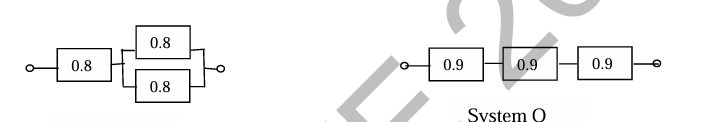
\includegraphics[width=\columnwidth]{q42.png}
        \caption*{}
        \label{fig:q42}
    \end{figure}
    
    The reliabilities of System P and System Q will be respectively
    
    \hfill{\brak{\text{GATE PI 2014}}}
    \begin{enumerate}
        \begin{multicols}{2}
            \item $0.768, 0.729$
            \item $0.512, 0.729$
            \item $0.5, 0.271$
            \item $0.232, 0.271$
        \end{multicols}
    \end{enumerate}

    \item Marks obtained by $100$ students in an examination are given in the table.
    
    \begin{table}[H]
        \centering
        \caption*{}
        \label{tab:q43}
        \begin{tabular}{ccc}
            \hline
            \textbf{Sl. No.} & \textbf{Marks Obtained} & \textbf{Number of Students} \\
            \hline
            1. & 25 & 20 \\
            2. & 30 & 20 \\
            3. & 35 & 40 \\
            4. & 40 & 20 \\
            \hline
        \end{tabular}
    \end{table}
    
    What would be the mean, median, and mode of the marks obtained by the students?
    
    \hfill{\brak{\text{GATE PI 2014}}}
    \begin{enumerate}
        \begin{multicols}{2}
            \item Mean $33$; Median $35$; Mode $40$
            \item Mean $35$; Median $32.5$; Mode $40$
            \item Mean $33$; Median $35$; Mode $35$
            \item Mean $35$; Median $32.5$; Mode $35$
        \end{multicols}
    \end{enumerate}

    \item In a given day in the rainy season, it may rain $70\%$ of the time. If it rains, chance that a village fair will make a loss on that day is $80\%$. However, if it does not rain, chance that the fair will make a loss on that day is only $10\%$. If the fair has not made a loss on a given day in the rainy season, what is the probability that it has not rained on that day?
    
    \hfill{\brak{\text{GATE PI 2014}}}
    \begin{enumerate}
        \begin{multicols}{4}
            \item $3/10$
            \item $9/11$
            \item $14/17$
            \item $27/41$
        \end{multicols}
    \end{enumerate}

    \item For the linear programming problem given below, find the number of feasible corner point solutions. Is the optimal solution degenerate?
    \begin{align*}
        \text{Maximize } & z = 2x_1 + 3x_2 \\
        \text{Subject to: } & x_1 + 2x_2 \leq 60; \\
        & 2x_1 + x_2 \leq 30; \\
        & x_1 - x_2 \geq -10; \\
        & x_1 \geq 0; \\
        & x_2 \geq 0
    \end{align*}
    
    \hfill{\brak{\text{GATE PI 2014}}}
    \begin{enumerate}
        \begin{multicols}{4}
            \item $4$; No
            \item $4$; Yes
            \item $5$; No
            \item $5$; Yes
        \end{multicols}
    \end{enumerate}

    \item A manufacturing company must select a process for its new product, VS-5, from among two alternatives. The following cost data have been gathered.
    \begin{table}[H]
        \centering
        \caption*{}
        \label{tab:q46}
        \begin{tabular}{ccc}
            \hline
            \textbf{Cost} & \textbf{Process X} & \textbf{Process Y} \\
            \hline
            Fixed & Rs. 10,000 & Rs. 40,000 \\
            Variable & Rs. 5/unit & Rs. 2/unit \\
            \hline
        \end{tabular}
    \end{table}
    If the objective is to select a process with the least total cost for a given demand, which one of the following is the most appropriate choice?
    
    \hfill{\brak{\text{GATE PI 2014}}}
    \begin{enumerate}
        \item Below $10,000$ units, Process X; Above $10,000$ units, Process Y
        \item Below $10,000$ units, Process Y; Above $10,000$ units, Process X
        \item Below $20,000$ units, Process X; Above $20,000$ units, Process Y
        \item Below $20,000$ units, Process Y; Above $20,000$ units, Process X
    \end{enumerate}

    \item The following data refers to a manufacturing plant.
    \begin{table}[H]
        \centering
        \caption*{}
        \label{tab:q47}
        \begin{tabular}{lcc}
            \hline
             & \textbf{Current Year} & \textbf{Previous Year} \\
            \hline
            Revenue generated \brak{\text{in Rs.}} & 200,000 & 220,000 \\
            Number of units produced & 1000 & 1200 \\
            Piece rate of workers \brak{\text{in Rs.}} & 22 & 18 \\
            \hline
        \end{tabular}
    \end{table}
    Assuming the previous year to be the base year, the labor productivity index for this plant is \underline{\hspace{2cm}}.
    
    \hfill{\brak{\text{GATE PI 2014}}}

    \item A manufacturing company producing ball bearings has conducted a time study for $10$ cycles of a job consisting of three elements. The details are shown in the table below.
    
    \begin{table}[H]
        \centering
        \caption*{}
        \label{tab:q48}
        \begin{tabular}{ccc}
            \hline
            \textbf{Job elements} & \textbf{Average elemental time \brak{\text{in minutes}}} & \textbf{Performance rating factor} \\
            \hline
            1 & 0.12 & 0.8 \\
            2 & 0.34 & 1.1 \\
            3 & 0.48 & 1.2 \\
            \hline
        \end{tabular}
    \end{table}
    
    If the permissible allowance is $15\%$, then the standard time \brak{\text{in minutes}} is \underline{\hspace{2cm}}.
    
    \hfill{\brak{\text{GATE PI 2014}}}

    \item A control chart for number of non-conformities per unit is to be constructed for a manufacturing process. Sixteen non-conformities were recorded while inspecting $30$ units. How should the Upper Control Limit \brak{UCL} and the Lower Control Limit \brak{LCL} be set for this control chart?
    
    \hfill{\brak{\text{GATE PI 2014}}}
    \begin{enumerate}
        \begin{multicols}{2}
            \item UCL = $1.81$, LCL = $0.70$
            \item UCL = $2.71$, LCL = $0.00$
            \item UCL = $0.533$, LCL = $-0.533$
            \item UCL = $3.10$, LCL = $-1.46$
        \end{multicols}
    \end{enumerate}

    \item For a given volume of a riser, if the solidification time of the molten metal in riser needs to be quadrupled, the surface area of the riser should be made
    
    \hfill{\brak{\text{GATE PI 2014}}}
    \begin{enumerate}
        \begin{multicols}{4}
            \item one-fourth
            \item half
            \item double
            \item four times
        \end{multicols}
    \end{enumerate}

    \item A $80$ mm thick steel plate with $400$ mm width is rolled to $40$ mm thickness in $4$ passes with equal reduction in each pass, by using rolls of $800$ mm diameter. Assuming the plane-strain deformation, what is the minimum coefficient of friction required for unaided rolling to be possible?
    
    \hfill{\brak{\text{GATE PI 2014}}}
    \begin{enumerate}
        \begin{multicols}{4}
            \item $0.111$
            \item $0.158$
            \item $0.223$
            \item $0.316$
        \end{multicols}
    \end{enumerate}
    
    \item In an arc welding operation, carried out with a power source maintained at $40$ volts and $400$ amperes, the consumable electrode melts and just fills the gap between the metal plates to be butt-welded. The heat transfer efficiency for the process is $0.8$, melting efficiency is $0.3$ and the heat required to melt the electrode is $20 \text{ J/mm}^3$. If the travel speed of the electrode is $4$ mm/s, the cross-sectional area, in mm$^2$, of the weld joint is \underline{\hspace{2cm}}.
    
    \hfill{\brak{\text{GATE PI 2014}}}
    
    \item A hard ceramic marble, having density \brak{\rho} of $3000 \text{ kg/m}^3$ and diameter \brak{d} of $0.025$ m, is dropped accidentally from a static weather balloon at a height of $1$ km above the roof of a greenhouse. The flow stress of roof material \brak{\sigma} is $2.5$ GPa. The marble hits and creates an indentation on the roof. Assume that the principle of creation of indentation is the same as that in case of abrasive jet machining \brak{AJM}. The acceleration due to gravity \brak{g} is $10 \text{ m/s}^2$. If V is the velocity, in m/s, of the marble at the time it hits the greenhouse, the indentation depth \brak{\delta = \frac{V}{1000} \times \sqrt{\frac{d\rho}{6\sigma}}}, in mm, is \underline{\hspace{2cm}}.
    
    \hfill{\brak{\text{GATE PI 2014}}}

    \item An HSS drill of $20$ mm diameter with $5$ mm cone height is used to drill a through hole in a steel work-piece of $50$ mm thickness. Cutting speed of $10$ m/min and feed rate of $0.3$ mm/rev are used. The drilling time, in seconds, neglecting the approach and over travel, is \underline{\hspace{2cm}}.
    
    \hfill{\brak{\text{GATE PI 2014}}}

    \item The alignment test "Spindle square with base plate" is applied to the radial drilling machine. A dial indicator is fixed to the cylindrical spindle and the spindle is rotated to make the indicator touch the base plate at different points. This test inspects whether the
    
    \begin{figure}[H]
        \centering
        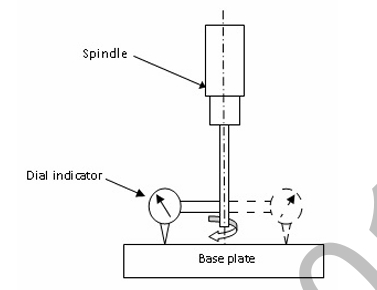
\includegraphics[width=0.4\columnwidth]{q55.png}
        \caption*{}
        \label{fig:q55}
    \end{figure}
    
    \hfill{\brak{\text{GATE PI 2014}}}
    \begin{enumerate}
        \item spindle vertical feed axis is perpendicular to the base plate
        \item axis of symmetry of the cylindrical spindle is perpendicular to the base plate
        \item axis of symmetry, the rotational axis and the vertical feed axis of the spindle are all coincident
        \item spindle rotational axis is perpendicular to the base plate
    \end{enumerate}

\end{enumerate}

\end{document}